
\documentclass[12pt]{article}
\usepackage[a4paper, top=1cm, right=1.5cm, bottom=1cm, left=1.5cm]{geometry}
\usepackage[onehalfspacing]{setspace}

\usepackage[utf8]{inputenc}
\usepackage[T1]{fontenc}
\usepackage{amsmath}
\usepackage{xargs}
\usepackage{tikz}
\usepackage{tabularx, multirow}


%\tgrph{ordre}[taille][rota(senstrigo)]
\newcommandx{\tgrph}[3][2=2, 3=0]{
\begin{tikzpicture}[thick, transform shape]
    \foreach \x in {1,...,#1}{
        \pgfmathparse{\x*(360/#1)-(360/#1)+90+#3}
        \node[draw,circle,minimum size=0.5cm] (N-\x) at (\pgfmathresult:#2cm) {\x};
    }
    \foreach \x [count=\xi from 1] in {2,...,#1}{
        \foreach \y in {\x,...,#1}{
            \draw (N-\xi) -- (N-\y);
        }
    }
\end{tikzpicture}
}

%\ct{elements}[columns]
\newcommandx{\ct}[2][2=ccc]{
    \begin{center}
        \begin{tabular}{#2}
            #1
        \end{tabular}
    \end{center}
}

%\db{elements}
\newcommandx{\db}[1]{
    Définition:

    \begin{tabularx}{\linewidth}{|X|}
        \hline
        #1\\
        \hline
    \end{tabularx}
}

%\pb{elements}
\newcommandx{\pb}[1]{
    Propriété:

    \begin{tabularx}{\linewidth}{|X|}
        \hline
        #1\\
        \hline
    \end{tabularx}
}

%\go{ordre}
\newcommandx{\go}[1]{
    \begin{tikzpicture}[node distance={15mm}, thick, main/.style = {draw, circle}]
        \node[main] (1) {1};
        \ifnum#1=1
        \else
            \foreach \x in {2,...,#1}{
                \node[main] (\x) [right of=\fpeval{\x-1}] {\x};
                \draw (\fpeval{\x-1}) -- (\x);
            }
        \fi
    \end{tikzpicture}
}


\begin{document}
    \begin{center}\Huge{\textbf{Chap 6 : Graphes}}\end{center}
    \setlength{\parindent}{0cm}
    \bgroup\obeylines

    \section{Introduction aux graphes}
        \subsection{Vocabulaire}
            \subsubsection{Graphe non-orienté}
                \db{Un graphe non-orienté G est un ensemble de sommets reliés par des arêtes.}
                \textit{Exemple:}
                \ct{
                    Sommet & Arête & Graphe G\\
                    \tikz[thick]\node[draw,circle](1){1}; & \tikz[thick]\draw(0,1)--(1,1); & \tgrph{2}[0.5][90]
                }

                \subsubsection{Adjacence et incidence}
                \db{Deux sommets reliés par une arête sont dits adjacents.
                    Une arête reliant deux sommets est dite incidente à ces deux sommets.
                    Une arête est une boucle si elle relie un sommet à lui-même.}
                \textit{Exemple:}
                \ct{
                    1 et 2 sont adjacents & L'arête est incidente à 1 & boucle\\
                    \tgrph{2}[0.5][90] & \tgrph{1}[1][90] & \tikz[thick]{\node[draw,circle](1){1};\draw(1)to[out=60,in=120,looseness=5](1);}
                }

                \subsubsection{Ordre et degré}
                \db{L'ordre d'un graphe est le nombre total de ses sommets.
                    Le degré d'un sommet est le nombre d'arêtes incidentes à ce sommet, les arêtes comptant pour deux.
                    Un graphe est dit simple si au plus une arête relie deux sommets et s'il n'y a pas de boucle sur un sommet.}
                \textit{Exemple:}
                \ct{
                    Graphe d'ordre 3 & 1 est de degré 2 & Graphe simple d'ordre 4\\
                    \go{3} & \tgrph{3}[0.75] & \go{4}
                }

                \pb{Soit G un graphe simple non-orienté, la somme du degré des sommets de G est égale au double du nombre d'arêtes de G.}


        \subsection{Graphes complets}
            \db{Un graphe non-orienté est dit complet si tous ses sommets sont adjacents.}
            \textit{Exemple:}
            \ct{
                Ordre 5 & Ordre 7 & Ordre 9\\
                \tgrph{5} & \tgrph{7} & \tgrph{9}
            }


        \subsection{Chaînes}
            \subsubsection{Chaînes}
            \subsubsection{Chaîne d'Euler}


    \section{Graphes orientés et lien avec les matrices}
        \subsection{Graphes orientés}
        \subsection{Matrices}
            \subsubsection{Matrice d'adjacence}
            \subsubsection{Puissances de matrices}


    \section{Pour aller plus loin}
        \subsection{Chaîne de Markov}

        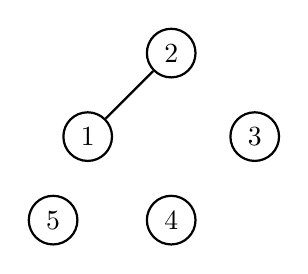
\begin{tikzpicture}[node distance={15mm}, thick, main/.style = {draw, circle}]
            \node[main] (1) {1};
            \node[main] (2) [above right of=1] {2};
            \node[main] (3) [below right of=2] {3};
            \node[main] (4) [below left of=3] {4};
            \node[main] (5) [left of=4]{5};
            \draw (1) -- (2);
        \end{tikzpicture}

    \egroup

    % \pagenumbering{}
\end{document}
